\documentclass[12pt]{article}

\usepackage{a4wide}
\usepackage[utf8]{inputenc}

\usepackage[percent]{overpic}
\usepackage{graphicx}
\usepackage{mathtools}
\usepackage{placeins}

\pagestyle{empty}

%\parindent=0pt

\def\mvec#1{\mathbf{#1}}

\begin{document}

\section*{Convolution}

In this exercise, we'll implement a convolution algorithm. Convolution is a mathematical operation on two functions
and produces a third function that is usually a modification of one of the original functions.
Convolution is often used to realise different filters of images.

In digital image processing, convolution usually takes the following form
\begin{equation}
    \label{eq:tri}
    (f * h)(x, y) = \sum\limits_{i=-k}^{k} \sum\limits_{j=-k}^{k} f(x - i, y - j) \cdot h(i, j) \, ,
\end{equation}
where $f$ is and input image, $h$ is a convolution matrix (mask), and $k$ is the width of the convolution mask.

Convolution mask is a matrix usually of size $3 \times 3$ or $5 \times 5$. Some examples of convolution masks follow:

\begin{equation}
    \label{eq:box_blur}
    \text{Box blur:} \quad\quad \frac{1}{9}
    \begin{bmatrix}
        1 & 1 & 1 \\
        1 & 1 & 1 \\
        1 & 1 & 1
    \end{bmatrix}
    \, ,
\end{equation}

\begin{equation}
    \label{eq:gauss_blur_3}
    \text{Gaussian blur $3 \times 3$:} \quad\quad \frac{1}{16}
    \begin{bmatrix}
        1 & 2 & 1 \\
        2 & 4 & 2 \\
        1 & 2 & 1
    \end{bmatrix}
    \, ,
\end{equation}

\begin{equation}
    \label{eq:gauss_blur_5}
    \text{Gaussian blur $5 \times 5$:} \quad\quad \frac{1}{256}
    \begin{bmatrix}
        1 & 4  & 6  & 4  & 1 \\
        4 & 16 & 24 & 16 & 4 \\
        6 & 24 & 36 & 24 & 6 \\
        4 & 16 & 24 & 16 & 4 \\
        1 & 4  & 6  & 4  & 1
    \end{bmatrix}
    \, .
\end{equation}

Convolution can be roughly transcribed as producing output image by adding each element of the image to its local neighbour pixel values, weighted by the mask.
If we look at the operation, it not possible to compute convolution on the image boundary. The size of the boundary is given by the mask size. For mask of size $3 \times 3$
the border is $1$ pixel, for mask of size $5 \times 5$ the border is $2$ pixels. In Fig. \ref{img:convolution_example}, an example of convolution operation is depicted.

\begin{figure}[th]
\begin{center}
    \begin{overpic}[width=0.8\textwidth,tics=5]{conv}
        \put (10, 55) {original image}
        \put (30, 48) {brightness}
        \put (35, 44) {values}
        \put (50, 43) {convolution}
        \put (55, 40) {mask}
        \put (80, 45) {result at pixel}
    \end{overpic}
    \caption{An example of convolution operation at a pixel location.}
    \label{img:convolution_example}
\end{center}
\end{figure}

%\begin{figure}[th}
%        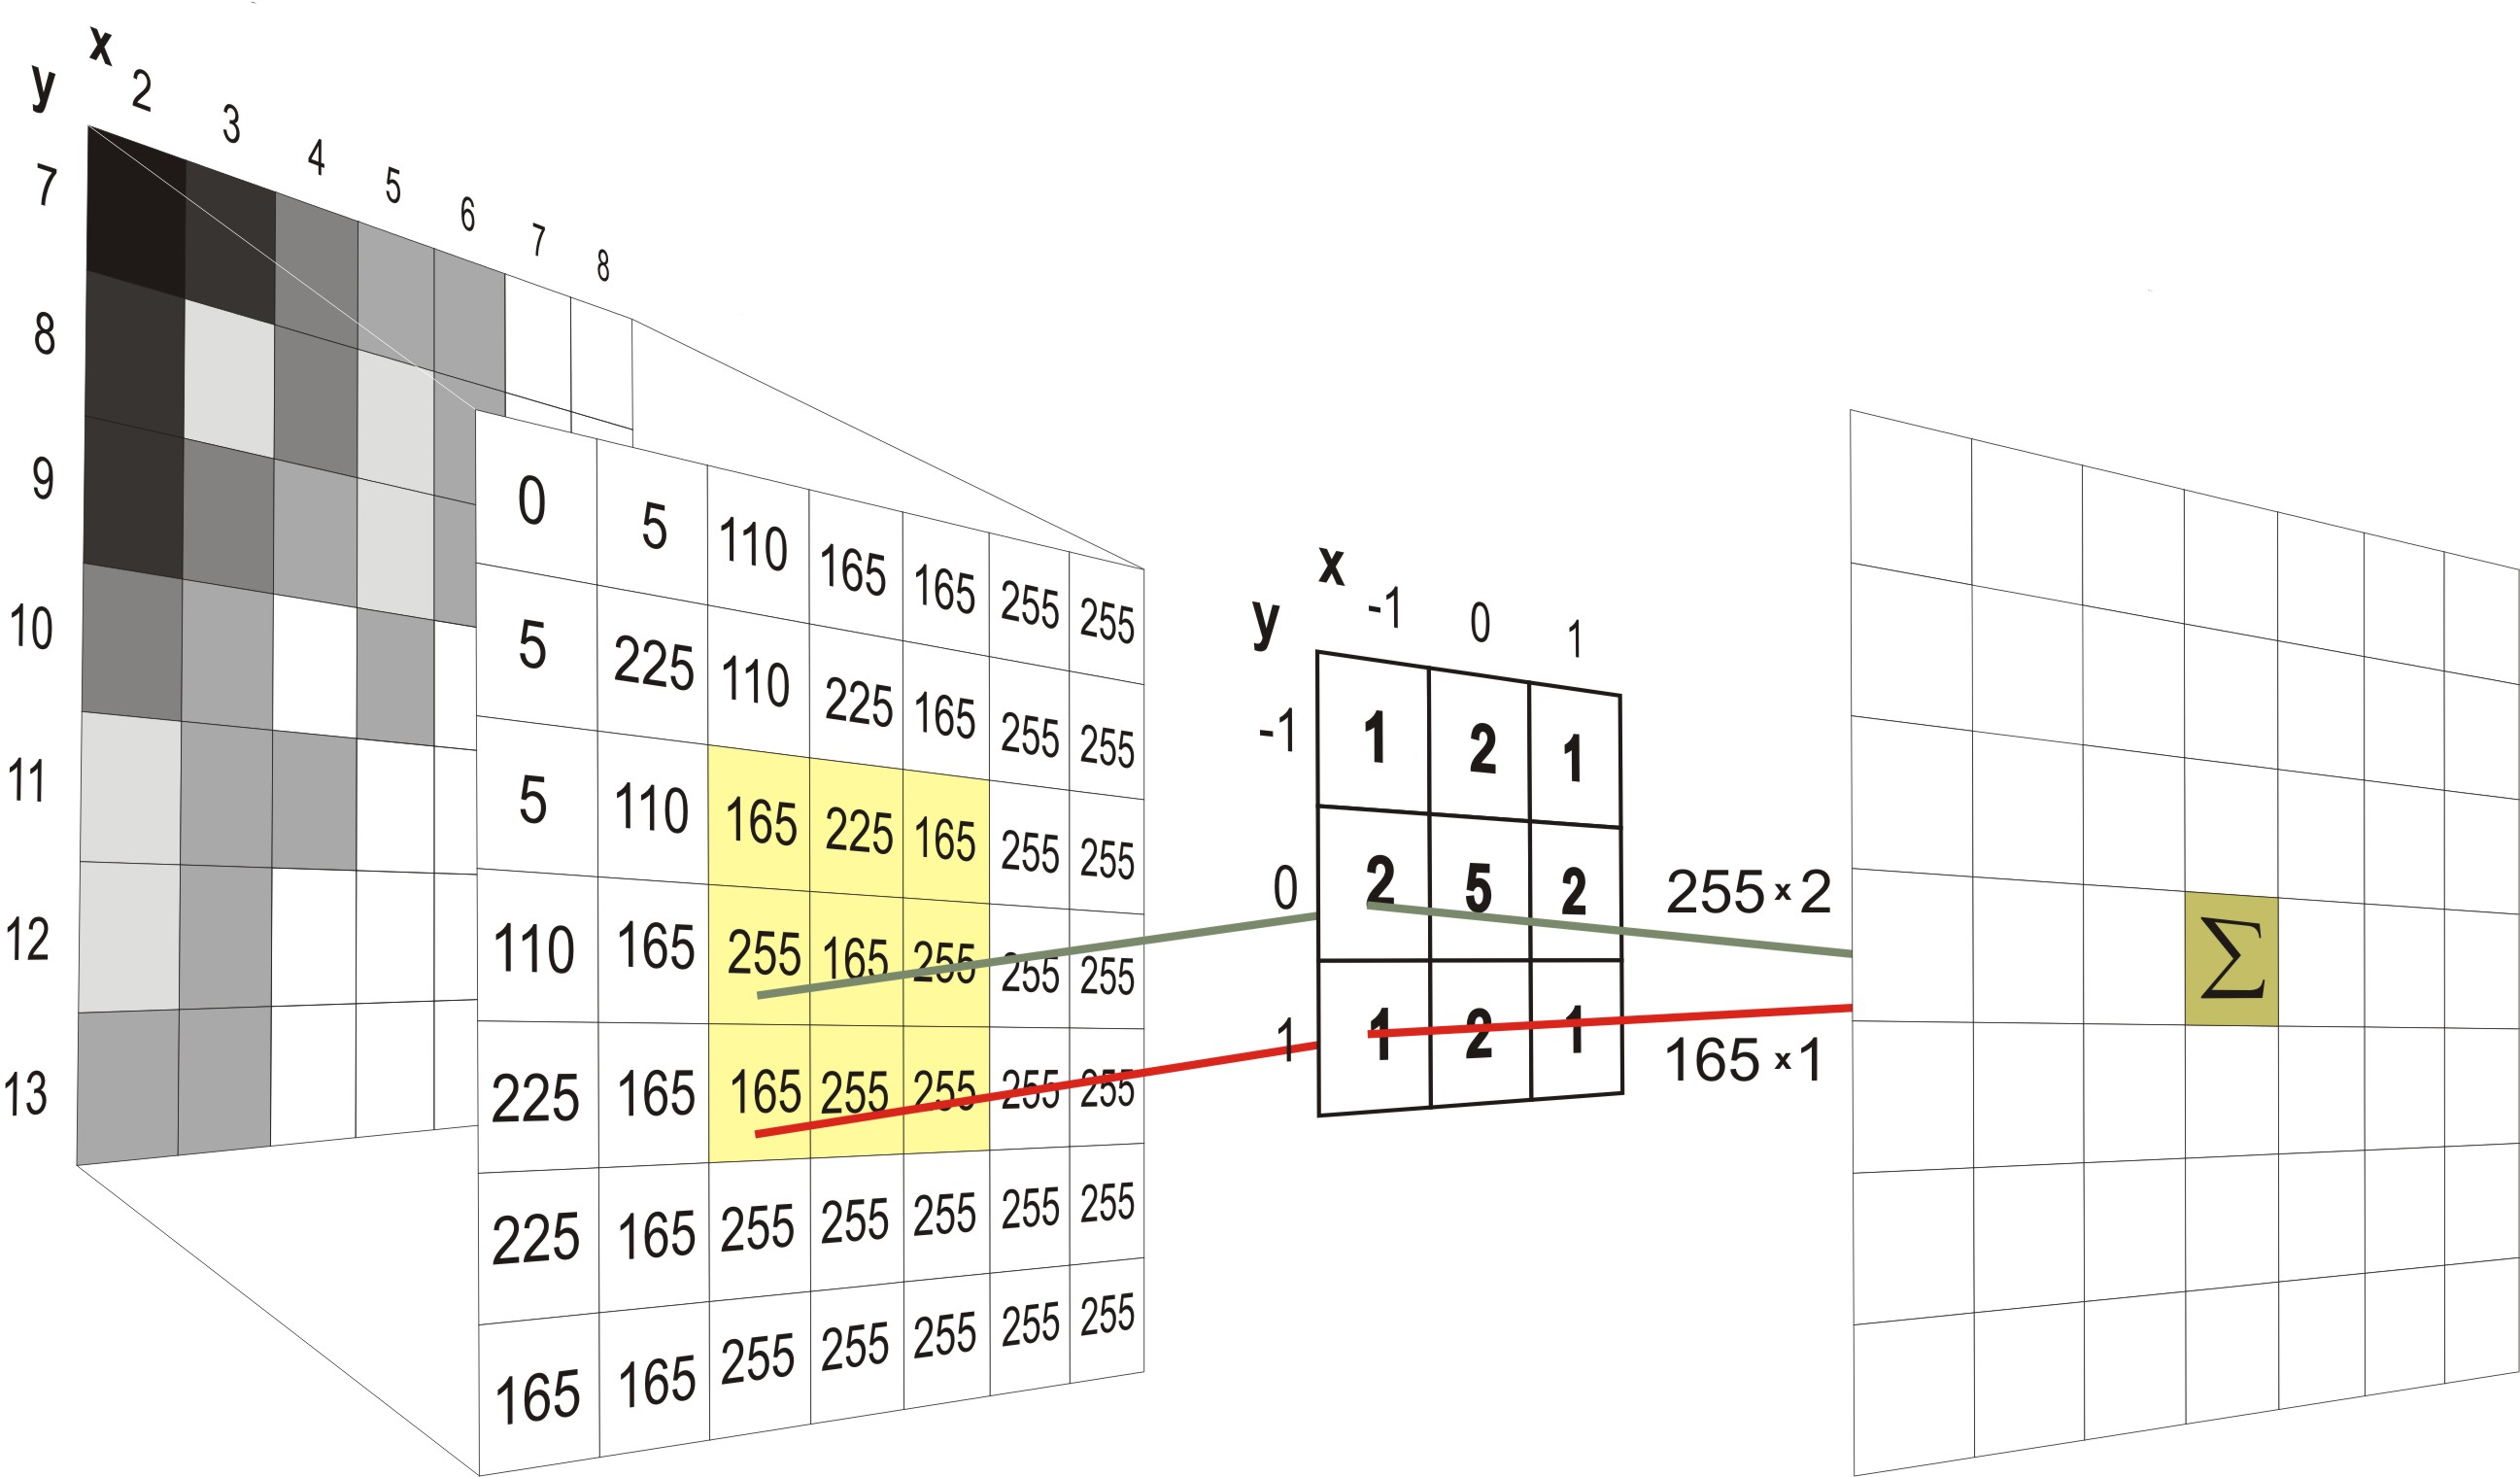
\includegraphics[width=0.8\textwidth]{conv.png}
%    \end{center}
%    \caption{An example of convolution operation at a pixel location.}
%    \label{img:convolution_example}
%\end{figure}


%\newpage

%\FloatBarrier
%\section*{Expected Output}

%\begin{figure}[h]
%    \centering
%    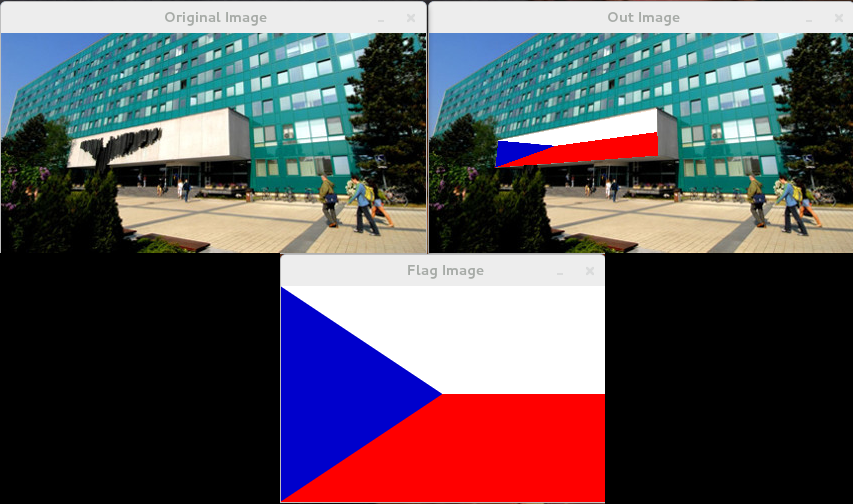
\includegraphics[width=0.8\textwidth]{persp_proj.png}
%    \caption{Input image (\textit{top left} and \textit{bottom} images); output image (\textit{top right} image).}
%    \label{fig:result}
%\end{figure}

\end{document}

